% Chapter: On the Recoverability of Coalescence Phase and Polarization Angle
% from Gravitational-Wave Strain: A Systematically Verified Null Result
%
% Requires (thesis preamble): amsmath, amssymb, booktabs, graphicx
% Figures are referenced from the experiment directory; adjust \graphicspath
% or copy the PNGs into the thesis figures/ directory.
%
% Draft status: chapter number, cross-references, and \cite keys are
% placeholders to be resolved against the thesis bibliography. All
% quantitative values are taken verbatim from the experiment record on
% branch poc/phic-psi-degeneracy (see the claim-to-artifact map in the
% chapter appendix).

\usepackage{geometry}
\usepackage{graphicx}
\usepackage{amssymb}
\usepackage{amsfonts}
\usepackage{booktabs}
\usepackage{amsopn}
\usepackage{amsmath}
\usepackage{amstext}

%\graphicspath{{../}{../diagnostic_output/}{../analysis_output/}{../lam0_ablation_output/}{../lam005_retune_output/}{../lam010_retune_output/}}


\chapter{On the Recoverability of Coalescence Phase and Polarization Angle from Gravitational-Wave Strain: A Systematically Verified Null Result}
\label{ch:phic-psi-degeneracy}


\section{Introduction}
\label{sec:phicpsi:intro}

Deep-learning approaches to gravitational-wave parameter estimation have matured rapidly, from early proof-of-concept classifiers~\cite{george2018deep} to amortized neural posterior estimators that approach the accuracy of stochastic-sampling pipelines~\cite{gabbard2022vitamin,dax2021dingo} at a fraction of their latency.
Most of this progress has concentrated on parameters that imprint strongly and non-degenerately on the observed strain: the chirp mass through the phase evolution~\cite{cutler1994gw}, the merger time through the temporal localization of the signal, the signal-to-noise ratio through overall amplitude, and the sky position through inter-detector time delays and antenna-pattern amplitudes.

Two extrinsic parameters have received far less attention as direct regression targets: the orbital phase at coalescence, $\varphi_c$, and the polarization angle, $\psi$.
There is a physical reason for this neglect.
For the dominant quadrupole ($\ell=2$, $|m|=2$) mode of a quasi-circular compact binary, the two polarization states are
\begin{equation}
    h_+ \propto (1+\cos^2\iota)\,\cos\!\bigl(2\varphi(t)+2\varphi_c\bigr),
    \qquad
    h_\times \propto 2\cos\iota\,\sin\!\bigl(2\varphi(t)+2\varphi_c\bigr),
\end{equation}
and the detector response mixes them through antenna patterns that depend on $2\psi$~\cite{cutler1994gw,sathyaprakash2009physics}.
In the face-on limit ($\cos\iota \to \pm 1$) the signal becomes circularly polarized and depends on $\varphi_c$ and $\psi$ only through a single combination --- effectively $\varphi_c \pm 2\psi$, with the sign set by the sign of $\cos\iota$ --- so the individual angles are exactly unidentifiable there, and only partially disentangled as the inclination moves toward edge-on.
Bayesian samplers absorb this structure into broad, multimodal joint posteriors~\cite{veitch2015lalinference}; a point-estimate regression network has no such refuge.

This chapter asks directly:
\begin{quote}
\itshape Can $\varphi_c$ and $\psi$ be recovered from strain alone by a deep neural network --- individually, or through their better-conditioned sum/difference combinations --- or is the degeneracy effectively exact for a realistic detection-scale population?
\end{quote}

The answer we converge on is a \textbf{null result}: across five trunk architectures, two head parameterizations, four values of a magnitude-regularization coefficient, and roughly nine full training campaigns, no model ever performed measurably better than random guessing on either angle, while the same networks simultaneously recovered chirp mass, merger time, signal-to-noise ratio, and sky position with high fidelity from the same shared features.

A null result of this kind is only as strong as the effort spent trying to break it.
The scientific contribution of this chapter is therefore twofold.
First, the null itself, defended against an explicit list of confounds: data-pipeline faults, loss-wiring faults, two genuine and initially invisible optimization pathologies (a saturating output activation and a gradient-attenuating normalization layer), architecture-specific artifacts, statistical flukes, and population heterogeneity.
Second, a methodological account of \emph{how} the null was established, because the investigation was repeatedly misled by aggregate metrics before converging on a mechanism-first diagnostic discipline and, ultimately, a pre-registered decision procedure with mechanically evaluated success criteria~\cite{nosek2018preregistration}.
Ruling out artifacts is not preamble to the result here; it \emph{is} the result.

The chapter is organized conventionally, with one deliberate exception.
Section~\ref{sec:phicpsi:problem} formalizes the problem and the circular-regression framework.
Section~\ref{sec:phicpsi:prereq} presents an analytic prerequisite study that motivated the sum/difference reparameterization.
Section~\ref{sec:phicpsi:methods} details the datasets, architectures, losses, and training protocol.
Section~\ref{sec:phicpsi:arc} --- the exception --- narrates the diagnostic arc: the two optimization pathologies that had to be found and fixed before any measurement of the degeneracy could be trusted.
Section~\ref{sec:phicpsi:results} presents the defended null result and its verification battery.
Section~\ref{sec:phicpsi:prereg} describes the pre-registered magnitude-penalty retune and its outcome.
Section~\ref{sec:phicpsi:discussion} discusses interpretation, limitations, and future work; Section~\ref{sec:phicpsi:conclusion} concludes.


\section{Problem Formulation}
\label{sec:phicpsi:problem}

\subsection{Targets and the degeneracy hypothesis}
\label{subsec:targets-and-the-degeneracy-hypothesis}

We consider a ten-parameter description of a compact binary coalescence signal injected into two-detector noise: chirp mass $\mathcal{M}$, mass ratio $q$, inclination $\iota$, coalescence phase $\varphi_c$, polarization angle $\psi$, declination, right ascension, injection time, merger time within the analysis window, and network signal-to-noise ratio.
Of these, seven are used as supervised regression targets (mass ratio and injection time are excluded; \S\ref{sec:phicpsi:dataset}).
The scientific targets are $\varphi_c \in [0, 2\pi)$, with period $2\pi$, and $\psi \in [0, \pi)$, with period $\pi$.
Inclination, chirp mass, merger time, SNR, and sky position are retained as \emph{control heads}: parameters trained through the identical pipeline whose success or failure calibrates what the network can extract from strain when information is present.

The \textbf{degeneracy hypothesis} under test is: \emph{$\varphi_c$ and $\psi$ carry no strain-only recoverable signal for this population, in this architecture and loss family} --- i.e., a point-estimating network can do no better than the optimal constant (or constant-per-mode) prediction, because for most of the population the likelihood constrains only a combination of the two angles, and the remaining direction is unconstrained.

The alternative hypothesis motivating the experimental design is that even if $\varphi_c$ and $\psi$ are individually unrecoverable, their \textbf{sum and difference combinations} may be well-conditioned: face-on systems constrain $\varphi_c \mp 2\psi$ (sign by $\cos\iota$), so a network parameterized in combination space, with a curriculum that weights each combination according to how well the current inclination constrains it, might learn the recoverable structure that a naive per-angle parameterization misses.

\subsection{Circular regression framework}
\label{sec:phicpsi:circular}

Periodic targets are regressed on the unit circle~\cite{mardia2000circular}.
An angle $\theta$ with period $T$ is encoded as the two-vector
\begin{equation}
    \mathbf{u}(\theta) = \bigl(\sin(2\pi\theta/T),\ \cos(2\pi\theta/T)\bigr),
\end{equation}
so the $\psi$ head, with $T=\pi$, physically encodes $2\psi$.
Each periodic head outputs a raw two-vector $\mathbf{v} \in \mathbb{R}^2$, projected onto the unit circle by a normalization layer, \texttt{normalize\_unit},
\begin{equation}
    \hat{\mathbf{u}} = \frac{\mathbf{v}}{\max(\lVert\mathbf{v}\rVert,\ \varepsilon)},
    \qquad \varepsilon = 10^{-8},
\end{equation}
and trained with the cosine (circular) loss
\begin{equation}
    \mathcal{L}_{\mathrm{circ}}
    = 1 - \hat{\mathbf{u}}_{\mathrm{pred}} \cdot \mathbf{u}_{\mathrm{true}}
    = 1 - \cos\Delta\theta .
    \label{eq:circloss}
\end{equation}
For uniformly distributed targets and any fixed prediction, the expected circular loss is exactly 1; the expected wrap-aware angular mean absolute error (ang\_MAE) is $T/4$ --- that is, $\pi/2 \approx 1.5708$\,rad for $\varphi_c$ and $\iota$, and $\pi/4 \approx 0.7854$\,rad for $\psi$.
These are the null baselines against which every result in this chapter is judged.

Two further diagnostic statistics recur throughout.
The \textbf{circular resultant} of a set of predicted angles, $r_{\mathrm{circ}} = \lVert \operatorname{mean}(\hat{\mathbf{u}}) \rVert$, measures mode collapse: $r_{\mathrm{circ}} \to 1$ means all predictions concentrate at one angle (the empirical baseline for our uniform targets is $r_{\mathrm{circ}} \approx 0.005$).
The \textbf{std\_ratio} of a head is the ratio of the standard deviation of its raw outputs to that of the encoded targets, accumulated over an epoch; because the targets lie on the unit circle, std\_ratio is a direct monitor of raw-magnitude health, with values far from unity signalling the pathology analyzed in \S\ref{sec:phicpsi:pathology2}.
We adopt $[0.5, 2.0]$ as the healthy band.

Non-periodic heads use a Huber loss ($\delta=1$) on transformed targets (log--$z$-scored chirp mass, $z$-scored SNR, sigmoid-bounded merger time), and the sky-position head uses a closed-form von Mises--Fisher negative log-likelihood on the unit sphere~\cite{fisher1953dispersion}.
All heads share a single trunk and are combined by learned homoscedastic uncertainty weighting~\cite{kendall2018multi}: each head $h$ carries a trainable log-variance $s_h$, clamped to $|s_h| \le 3$, contributing $e^{-s_h}\mathcal{L}_h + s_h$ to the total loss.


\section{Analytic Prerequisite Study}
\label{sec:phicpsi:prereq}

Before any training, the combination-space hypothesis was tested analytically on the dataset itself, using a toy detector-response model: for a sweep of inclinations, we computed the correlation between strain-derived quantities and each candidate combination, $A = \varphi_c + 2\psi$ and $B = \varphi_c - 2\psi$, and formed the ratio of the better-correlated (``well-constrained'') to the worse-correlated combination.

The definitive 100-point inclination sweep (50 points per sign of $\cos\iota$, 200 sky positions, 5{,}000-draw bootstrap) gave an unambiguous, sign-symmetric structure (Fig.~\ref{fig:phicpsi:sweep}):
\begin{itemize}
\item for $\cos\iota > 0$, combo $B$ is the better-constrained combination at \textbf{50 of 50} inclination points; for $\cos\iota < 0$, combo $A$ wins 50 of 50 --- a clean sign flip, as the circular-polarization picture predicts;
\item the preference ratio is strongest face-on, $\approx 1.56\times$, decaying monotonically toward $\approx 1.05$--$1.08\times$ at edge-on, never crossing 1.0 (minimum 1.049 at $\iota = 1.62$);
\item population-bootstrapped mean ratios are $1.155\times$ (95\% CI $[1.118, 1.195]$) for $\cos\iota > 0$ and $1.171\times$ (95\% CI $[1.130, 1.216]$) for $\cos\iota < 0$ --- modest but statistically unambiguous.
\end{itemize}

\begin{figure}[tbp]
    \centering
    
\includegraphics[width=\textwidth]{sweep_1_1_ratio_vs_iota.png}
    \caption[Analytic check of the $\varphi_c$--$\psi$ degeneracy
    structure]{Analytic check of the $\varphi_c$--$\psi$ degeneracy
    structure: ratio of the strain correlation with the well-constrained
    combination to the poorly-constrained one, as a function of
    inclination, for $\cos\iota > 0$ (left; combo $B = \varphi_c - 2\psi$
        favored) and $\cos\iota < 0$ (right; combo $A = \varphi_c + 2\psi$
        favored). Face-on systems prefer the expected combination by
        $\approx 1.56\times$; the preference shrinks to
        $\approx 1.05$--$1.08\times$ at edge-on but never inverts. Bootstrap
        means: $1.155\times$ (95\% CI $[1.118, 1.195]$) and $1.171\times$
        (CI $[1.130, 1.216]$).}
    \label{fig:phicpsi:sweep}
\end{figure}

The same study produced the curriculum weight: a Jacobian-conditioning derivation (finite-difference Jacobian of the angle-to-response map, condition number averaged over sky positions, interpolated on $\cos^2\iota$) yielded an empirical weight with $w(\text{face-on}) = 0.0000$ and $w(\text{edge-on}) = 0.1212$ after an earlier polynomial fit was rejected for producing negative weights (maximum residual 1.32, $w(\text{face-on}) = -5.29$ from the fit against 0.000 from the raw data).
The trained runs use the analytically motivated fallback
\begin{equation}
    w(\iota) = 1 - \cos^2\iota = \sin^2\iota,
    \label{eq:curriculum}
\end{equation}
which shares the fitted weight's essential feature (zero weight where the degeneracy is exact, maximal weight edge-on) while avoiding the fit's pathologies; the fitted variant was derived and validated but never wired into training, a caveat noted in \S\ref{sec:phicpsi:threats}.
Population balance was also confirmed: 28.7\% of samples are near-face-on ($|\cos\iota| > 0.9$) and 32.7\% near-edge-on ($|\cos\iota| < 0.5$), so neither regime is vanishingly rare.

The prerequisite study's gate verdict was GO: the combination structure exists in the data, with the predicted sign behavior.
Whatever the networks subsequently failed to learn, they did not fail for want of an analytically real target.


\section{Methods}
\label{sec:phicpsi:methods}

\subsection{Dataset}
\label{sec:phicpsi:dataset}

All experiments use a single pre-generated HDF5 dataset of simulated two-detector observations: \textbf{25{,}000 training and 5{,}000 validation samples}, each a pair of 4{,}096-sample noisy strain series for the H1 and L1 detectors --- a 2\,s window at 2048\,Hz --- stacked as a $(4096, 2)$ input tensor.
The merger is placed at 1.6--1.8\,s (80--90\% of the window).
Marginal parameter distributions (verified empirically; \S\ref{sec:phicpsi:suite}, Check~1): chirp mass 8.84--43.45\,$M_\odot$, mass ratio 0.20--1.00, network SNR uniform in $[7, 15]$, and --- critically --- $\varphi_c$, $\psi$, $\iota$, and right ascension uniform over their supports, with declination following the cos-weighted sky prior.
Strain is fed raw; the first layer of every trunk is a batch-normalization layer.
Targets are transformed per \S\ref{sec:phicpsi:circular}; transform statistics are fitted on the training split only.
No data augmentation or SNR-dependent sample weighting is used.

\subsection{Trunk architectures}
\label{sec:phicpsi:trunks}

Five one-dimensional trunk architectures were evaluated, all mapping the $(4096, 2)$ input to a pooled feature vector shared by every head (Table~\ref{tab:phicpsi:trunks}).
Each head is a two-layer MLP (64 hidden units, ReLU) on the shared features, with a linear 2-unit output for periodic heads (\S\ref{sec:phicpsi:pathology1} explains why \emph{linear}, not bounded, matters).
The five trunks were not chosen as a random sample of model space but as five distinct \emph{inductive-bias families} --- full-receptive-field dilated temporal convolution, plain hierarchical convolution, attention-based sequence modeling, explicit multi-scale kernels, and deep residual feature learning --- so that each represents a different hypothesis about how phase information might be encoded in the strain; the sufficiency of this pool for a null claim is argued in \S\ref{sec:phicpsi:pool}.

\begin{table}[tbp]
    \centering
    \caption{Trunk architectures.}
    \label{tab:phicpsi:trunks}
    \small
    \begin{tabular}{@{}lllc@{}}
        \toprule
        Trunk                    & Body                                                                      & Readout           & Feat.\ dim \\
        \midrule
        \texttt{tcn} (primary)   & conv stem (64ch, $k{=}7$, s2) $+$ 10 residual TCN blocks, & GAP $\oplus$ GMP & 128 \\
        & dilations 1--512, receptive field $\approx$ full window~\cite{bai2018tcn} &                   &            \\
        \texttt{cnn\_baseline}   & $4\times$ [Conv1D($k{=}16$) $\to$ BN $\to$ ReLU $\to$ MaxPool(4)] & GAP & 128 \\
        \texttt{cnn\_attention}  & 5 strided conv stages $\to$ 2 transformer blocks                          & attention pooling & 128 \\
        & ($d{=}128$, 4 heads)~\cite{vaswani2017attention}                          &                   &            \\
        \texttt{inception\_time} & conv stem (s4) $+$ 6 Inception modules,                                   & GAP               & 128        \\
        & kernels \{9, 19, 39\}~\cite{fawaz2019inceptiontime}                       &                   &            \\
        \texttt{resnet1d}        & 3 stages, filters 64/128/256, dilated blocks~\cite{he2016resnet} & GAP $\oplus$ GMP & 512 \\
        \bottomrule
    \end{tabular}
\end{table}

\subsection{Head parameterizations under test}
\label{sec:phicpsi:modes}

Two parameterizations of the $\varphi_c/\psi$ problem were crossed with the trunks:
\begin{description}
\item[baseline mode] independent circular-loss heads directly on $\varphi_c$ and $\psi$, each with its own uncertainty weight.
\item[poc mode (\texttt{SumDiffTrainer})] the $\varphi_c$ and $\psi$ heads are retained as raw outputs, unit-normalized, and combined by complex multiplication into the two combination vectors, $\mathbf{z}_A = \mathbf{z}_{\varphi_c} \otimes \mathbf{z}_{2\psi}$ (angle $\varphi_c + 2\psi$) and $\mathbf{z}_B = \mathbf{z}_{\varphi_c} \otimes \overline{\mathbf{z}_{2\psi}}$ (angle $\varphi_c - 2\psi$).
The circular loss is applied to the \emph{combinations}, per-sample weighted by the sign-dependent curriculum: with $\cos\iota \ge 0$, combo $B$ receives weight 1 and combo $A$ receives $w(\iota) = \sin^2\iota$; the roles swap for $\cos\iota < 0$.
The individual $\varphi_c/\psi$ uncertainty weights are removed and replaced by per-combo weights.
\end{description}

Named configurations referenced throughout: \textbf{poc\_a} $=$ baseline mode on the TCN trunk; \textbf{poc\_b} $=$ poc mode on the TCN trunk; \texttt{tcn}, \texttt{cnn\_baseline}, \texttt{cnn\_attention}, \texttt{inception\_time}, \texttt{resnet1d} $=$ baseline mode on the named trunk.
(poc\_a and \texttt{tcn} are identical in trunk and mode and differ only in run identity --- a deliberate seed-free replication pair.)

\subsection{Magnitude penalty}
\label{sec:phicpsi:magpen}

Following the diagnosis in \S\ref{sec:phicpsi:pathology2}, all main-line configurations add an explicit radial regularizer on the \emph{raw, pre-normalization} periodic outputs:
\begin{equation}
    \mathcal{L}_{\mathrm{mag}}
    = \lambda \sum_{\mathbf{v} \in \{\mathbf{z}_{\varphi_c},\, \mathbf{z}_{\psi}\}}
    \operatorname{mean}\!\bigl[(\lVert\mathbf{v}\rVert - 1)^2\bigr],
    \label{eq:magpen}
\end{equation}
the standard companion of cosine-similarity losses in metric learning.
$\lambda$ values of 0 (ablation), 0.01 (main runs), 0.05, and 0.10 (pre-registered retune) were tested.

\subsection{Training protocol}
\label{sec:phicpsi:protocol}

All runs share: Adam, initial learning rate $10^{-3}$, reduce-on-plateau schedule (factor 0.5, patience 5), batch size 128, \textbf{80 epochs}, seed 42, no early stopping, uncertainty weighting with log-variance clamp $\pm 3$, Huber $\delta = 1$.
Configuration differences are confined to the trunk, the loss mode, and $\lambda$, with three caveats recorded for honesty: the \texttt{cnn\_baseline}, \texttt{inception\_time}, and \texttt{resnet1d} configs omit the magnitude penalty ($\lambda = 0$) so the five-architecture comparison is not $\lambda$-matched; the two CNN configs use a smaller learning-rate floor ($10^{-7}$ vs $10^{-6}$); and \texttt{resnet1d} alone uses a 5-epoch warmup.
None of these differences touches the four models (poc\_a, poc\_b, tcn, cnn\_attention) on which the verified null (\S\ref{sec:phicpsi:results}) rests, which are $\lambda$-matched at 0.01.

\subsection{Evaluation}
\label{sec:phicpsi:evaluation}

Point predictions on the 5{,}000-sample validation set are scored by wrap-aware angular MAE (\S\ref{sec:phicpsi:circular}), $r_{\mathrm{circ}}$, and, for scalar heads, MAE/$R^2$.
Statistical significance of any apparent sub-null ang\_MAE is assessed by a label-permutation bootstrap (\S\ref{sec:phicpsi:bootstrap}): the observed ang\_MAE is compared against the distribution obtained from \textbf{10{,}000 random permutations} of the true labels against fixed predictions, which preserves both marginals while destroying any input--label association.
Population heterogeneity is probed by SNR-tercile stratification (\S\ref{sec:phicpsi:snr}).
A seven-check diagnostic suite (\S\ref{sec:phicpsi:suite}) instruments the data pipeline, loss wiring, uncertainty-weight trajectories, gradient routing, output saturation, the full gradient chain through the circular-loss pipeline, and early-training dynamics.


\section{The Diagnostic Arc: Making the Measurement Trustworthy}
\label{sec:phicpsi:arc}

The headline result of this chapter is that nothing was learned about $\varphi_c$ and $\psi$.
The first result obtained, however, was that \emph{something appeared to be learned} --- and the road from the first to the second is where most of the experimental effort was spent.
We narrate it explicitly, because two genuine optimization pathologies had to be discovered, mechanistically understood, and fixed before flat loss curves could be read as evidence about physics rather than as engineering failure; and because the record of misreadings corrected along the way is the strongest argument that the final reading is not itself one of them.

\subsection{Round 1: apparent success, actual collapse}
\label{sec:phicpsi:round1}

The first full campaign (seven configurations across the five trunks) produced a beguiling number: validation $R^2 = 0.754$ for $\psi$ in the poc-mode model.
It was an artifact.
Every $\varphi_c$ prediction across the TCN variants had collapsed to a single constant ($315^\circ$; $\psi$ collapsed to $67.5^\circ$), with circular resultant $r_{\mathrm{circ}} = 1.000$.
For a \emph{periodic} target with uniform truth and constant prediction, the expected ``$R^2$'' computed on wrapped residuals is not 0 but exactly
\begin{equation}
    R^2_{\mathrm{null}} = 1 - \frac{\pi^2/48}{\pi^2/12} = 0.75,
\end{equation}
so 0.754 was the signature of total mode collapse, not of learning.
Meanwhile the same models' chirp-mass heads reached $R^2 > 0.95$ --- the trunk was healthy; the periodic heads specifically were dead.
This was the first of several instances in which an aggregate metric, read naively, pointed in exactly the wrong direction, and it set the tone for everything that followed: \emph{no metric was thereafter trusted until the mechanism producing it was inspected.}

\subsection{The diagnostic suite}
\label{sec:phicpsi:suite}

Seven mechanism-level checks were built incrementally during the bug hunt and re-run against every subsequent campaign: (1) true-label distribution audit; (2) loss-wiring verification; (3) uncertainty-weight and loss trajectories; (4) gradient routing --- do the periodic head weights actually change after a training step; (5) output-saturation dump; (6) end-to-end gradient-chain trace through normalization, complex multiplication, curriculum weighting, and uncertainty scaling; (7) initialization-time saturation timing.

Check~1 immediately ruled out the data pipeline: true $\varphi_c/\psi/\iota$ are uniform to $r_{\mathrm{circ}} \le 0.013$ with no duplicated or quantized values (Fig.~\ref{fig:phicpsi:labels}).
Check~2 caught a real but benign wiring fault (stale Huber-loss registrations for $\varphi_c/\psi$ alongside the poc-mode combo losses --- never invoked, but removed).
Check~4 then produced the first smoking gun: after one optimizer step, every head's predictions moved \emph{except} $\varphi_c$ and $\psi$ (mean absolute prediction change 0.15--0.81 for scalar heads, \textbf{0.00} for both angles), while --- the crucial control --- the inclination head, which shares the trunk, the two-vector encoding, and the head architecture, moved healthily.
Whatever was killing $\varphi_c/\psi$ was in their final layer, not in the trunk or the data.

\begin{figure}[tbp]
    \centering
    \includegraphics[width=\textwidth]{true_label_distributions.png}
    \caption[True label distributions]{True label distributions after HDF5
    load, before target transforms, for training (top, $n = 25{,}000$) and
    validation (bottom, $n = 5{,}000$). $\varphi_c$, $\psi$, $\iota$, and
    right ascension are uniform over their supports (circular resultant
        $\le 0.013$); declination follows the non-uniform sky prior. The
        prediction collapse observed in training is not a data-pipeline
        artifact.}
    \label{fig:phicpsi:labels}
\end{figure}

\subsection{Pathology I: output saturation at initialization}
\label{sec:phicpsi:pathology1}

Check~6's forward-pass dump found the mechanism.
Every sample's raw $\varphi_c$ output was exactly $(-1.000000, +1.000000)$ --- norm $\sqrt{2} = 1.4142$ --- and had been from \textbf{step~0}: the periodic heads used a $\tanh$ output activation, and at random initialization the pre-activation logits were already large enough to saturate it.
At saturation $\tanh' \approx 0$, so although the gradient flowing \emph{into} the output was healthy ($\lVert \partial\mathcal{L}/\partial \mathbf{z}_{\mathrm{raw}} \rVert \approx 0.31$), the gradient reaching the weights was numerically zero (kernel gradient 0.000000; bias $3.7 \times 10^{-10}$).
Adam's momentum still moved the weights (kernel change of 2.46 after a step) without ever changing the predictions --- the model was, in the log's phrase, \emph{born dead}.
The constant $\sqrt{2}$ also retro-explained the frozen std\_ratio $= 1.4142$ seen in every earlier trajectory.

The fix is disproportionately small for the damage caused: the $\tanh$ was \textbf{redundant} --- \texttt{normalize\_unit} already projects onto the unit circle --- so the periodic output activations were changed to linear, and all seven configurations retrained.
Two lessons carried forward.
First, the saturation was invisible to every aggregate metric and to a logit-magnitude heuristic (an earlier check had ``ruled out'' saturation from an estimated logit scale; the direct dump proved the estimate wrong) --- only inspection of actual forward-pass values settled it.
Second, a redundant nonlinearity that is merely useless in expectation can be fatal in the tail of initialization space.

\subsection{Pathology II: normalization-induced magnitude drift}
\label{sec:phicpsi:pathology2}

The retrained models still did not learn the angles --- but now for a different, equally mechanical reason.
The backward pass of $\hat{\mathbf{u}} = \mathbf{v}/\lVert\mathbf{v}\rVert$ scales angular gradients by $1/\lVert\mathbf{v}\rVert$, and the circular loss, computed entirely on $\hat{\mathbf{u}}$, is \emph{blind} to $\lVert\mathbf{v}\rVert$: nothing in the objective anchors the raw magnitude.
Freed from $\tanh$'s box, $\lVert\mathbf{v}\rVert$ drifted unboundedly --- by epoch 79 the $\varphi_c$ head's std\_ratio reached \textbf{103.7} (gradients attenuated ${\sim}100\times$) and $\psi$'s $\approx 13$.
The pathology had been introduced \emph{by an earlier correct fix}: replacing an anisotropic Huber-on-vector loss (whose minimum at $\lVert\mathbf{v}\rVert = 1$ had implicitly regularized magnitude) with the isotropic circular loss silently discarded that side effect.
The remedy (\S\ref{sec:phicpsi:magpen}) is the standard explicit penalty $\lambda(\lVert\mathbf{v}\rVert - 1)^2$, adopted at $\lambda = 0.01$.

One misreading from this period required formal retraction and is retained in the record.
The inclination head appeared to fail ``identically'' to $\varphi_c/\psi$ and was briefly cited as key evidence that the collapse was a shared \texttt{normalize\_unit} bug rather than physics.
A code-level trace disproved this: the inclination head is trained with a \emph{Huber} loss on its raw two-vector --- no \texttt{normalize\_unit} in its path at all --- so its failure has a different (still unresolved) mechanism, plausibly convergence to the dataset-mean vector as Huber's optimal constant predictor, and is evidence \emph{neither for nor against} the $\varphi_c/\psi$ mechanism.
The control that seemed to prove the point was not a valid control; only code inspection, not metric comparison, revealed this.

\subsection{Run 7: healthy machinery, flat objective}
\label{sec:phicpsi:run7}

With linear outputs and the $\lambda = 0.01$ penalty, the four $\lambda$-matched models (poc\_a, poc\_b, tcn, cnn\_attention) were retrained and re-instrumented.
The machinery now verifiably works: raw magnitudes contract from initialization norms of ${\sim}100$--250 to $\lVert\mathbf{v}\rVert \approx 1$ by epoch ${\sim}40$; gradient norms at the periodic head kernels are 0.58--1.37 (previously 0.0); predictions move after an optimizer step (mean $|\Delta| \approx 1.4$--$1.5 \times 10^{-2}$); and the epoch-79 std\_ratio sits at order unity for most model--head pairs (poc\_b 0.85/0.67, cnn\_attention 0.64/0.62, poc\_a 0.69/0.44, tcn 0.34/0.62 for $\varphi_c/\psi$ respectively).

And yet: \textbf{validation circular loss for every periodic head, in every model, sat at the random-guessing value $\approx 1.0$ for all 80 epochs} (Fig.~\ref{fig:phicpsi:comboloss}) --- poc\_a $\varphi_c$ $0.995 \to 1.020$, $\psi$ $0.990 \to 1.006$; tcn $0.995 \to 1.016$ and $0.992 \to 1.006$; poc\_b's \emph{combination} losses likewise (combo $A$ $0.999 \to 0.999$, combo $B$ $1.006 \to 0.991$).
Crucially, the loss stayed flat even during epochs 40--79 when $\lVert\mathbf{v}\rVert \approx 1$ and gradient flow was demonstrably healthy --- the strongest mechanistic evidence that the remaining failure is not an optimization artifact.
Higher-capacity trunks did \emph{reduce training} circular loss substantially (to $\approx 0.49$--0.60 for cnn\_baseline, cnn\_attention, resnet1d) with validation pinned at 1.0 throughout: they memorized the training set's phase labels, the behavior expected of a flexible model given a target that is unpredictable from its input.

\begin{figure}[tbp]
    \centering
    \includegraphics[width=\textwidth]{combo_loss_trajectories.png}
    \caption[Circular-loss trajectories, all architectures]{Circular-loss
        ($1 - \cos\Delta\theta$) trajectories for $\varphi_c$ and $\psi$
        (combo $A$/$B$ for poc\_b) across all seven architectures.
        Higher-capacity models memorize the training set --- training loss
        falls as low as $\approx 0.49$ --- while validation loss stays pinned
        at the random-guessing value $\approx 1.0$ in every case: the
        signature of a target unpredictable from the input, not of an
        optimization failure.}
    \label{fig:phicpsi:comboloss}
\end{figure}

The learned uncertainty weighting corroborates this reading from a different direction (Fig.~\ref{fig:phicpsi:logvar}): the well-learned scalar heads rapidly acquire large effective weights ($e^{-s} > 20$ for chirp mass and merger time), while the periodic heads' weights stay near unity --- the multi-task machinery correctly identifies them as uninformative rather than starving them of gradient.

\begin{figure}[tbp]
    \centering
    \includegraphics[width=\textwidth]{logvar_trajectories.png}
    \caption[Uncertainty-weighting trajectories]{Uncertainty-weighting
    trajectories $e^{-s_h}$ per head for all seven architectures. Scalar
    heads that learn (chirp mass, merger time) acquire large weights; the
        $\varphi_c/\psi$ heads (and poc\_b's combo heads, flat at
        $\approx 1.3$) remain near unity.}
    \label{fig:phicpsi:logvar}
\end{figure}

\subsection{Positive controls}
\label{sec:phicpsi:controls}

The same checkpoints recover the control parameters well (Fig.~\ref{fig:phicpsi:mchirp}): chirp mass $R^2 = 0.926$--0.963 (MAE 0.95--1.36\,$M_\odot$), merger time $R^2 = 0.909$--0.921, SNR $R^2 = 0.755$--0.785, and sky position to $3.3^\circ$--$10.0^\circ$ mean angular error (median $0.0^\circ$) --- with cnn\_attention, the \emph{worst} periodic-head model by ang\_MAE, achieving the \emph{best} sky localization ($3.3^\circ$).
Information that is present in the strain is extracted by this pipeline; the two phase angles specifically are not.

\begin{figure}[tbp]
    \centering
    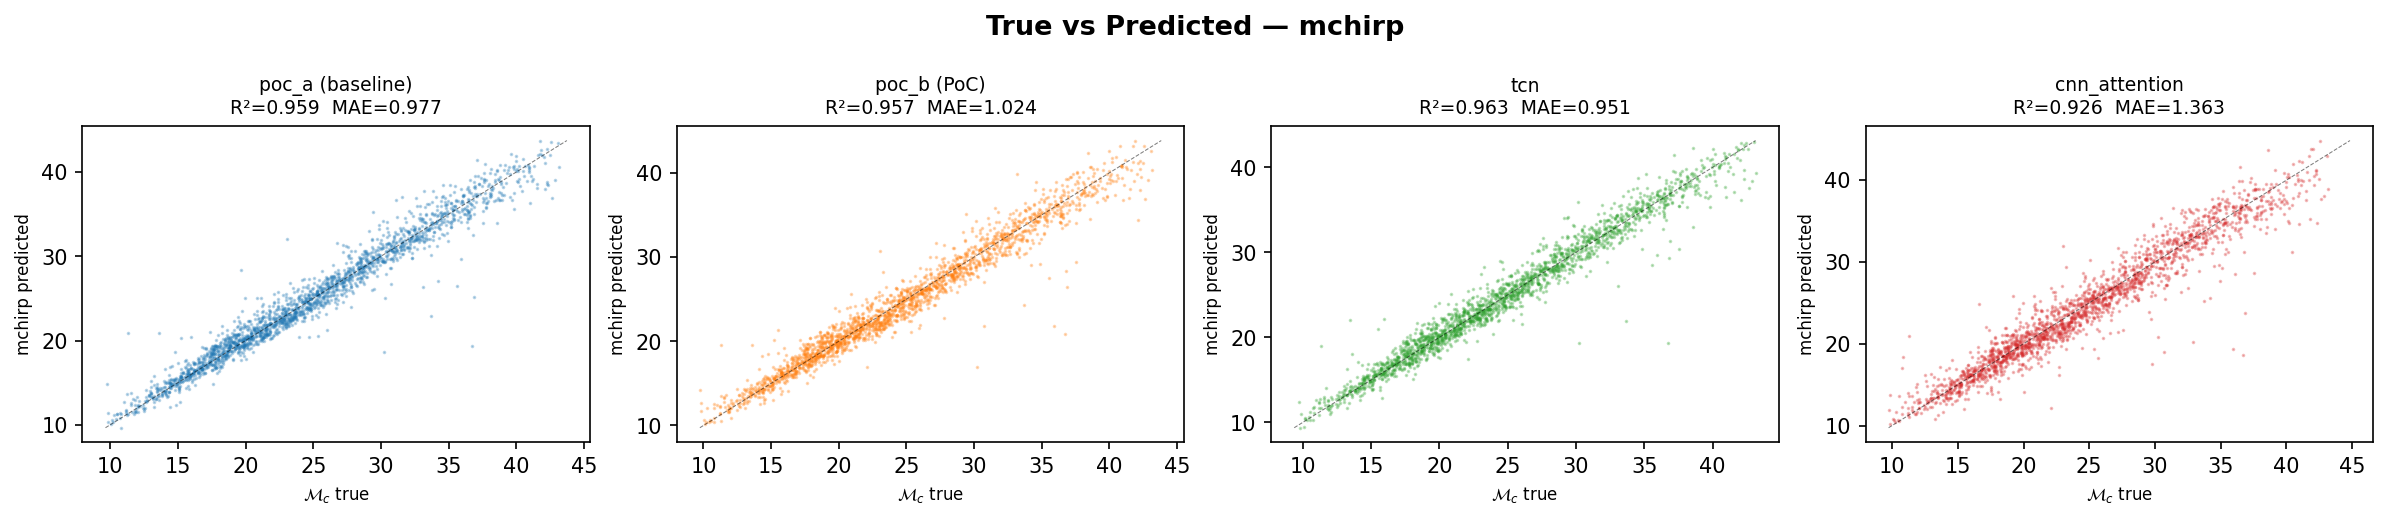
\includegraphics[width=\textwidth]{scatter_mchirp_20260720_234304.png}
    \caption[Chirp-mass recovery (positive control)]{Chirp-mass recovery on the validation set for the four Run~7 models ($R^2 = 0.93$--0.96).
    Together with merger time, SNR, and sky position, these positive controls establish that the shared trunk and training pipeline learn strain-derived parameters when the information is present.}
    \label{fig:phicpsi:mchirp}
\end{figure}


\section{Results: A Defended Null}
\label{sec:phicpsi:results}

\subsection{Headline result}
\label{subsec:headline-result}

Table~\ref{tab:phicpsi:prepost} collects the final validation angular MAE for every architecture, before and after the activation fix, against the analytic null.
The values are not merely \emph{close to} the null; they bracket it within a few hundredths of a radian in both directions, across seven architectures, two head parameterization, and every $\lambda$.

\begin{table}[tbp]
    \centering
    \caption{Validation angular MAE (rad) against the random-guessing
    null. ``Pre'' $=$ $\tanh$ outputs, Round~1; ``post'' $=$ linear
    outputs with $\lambda = 0.01$ where configured, Run~7 era. Dashes: no
    pre-fix run.}
    \label{tab:phicpsi:prepost}
    \small
    \begin{tabular}{@{}lccccccc@{}}
        \toprule
        Head (null)             & TCN   & ResNet1D & CNN base & CNN attn & Inception & poc\_a & poc\_b \\
        \midrule
        $\varphi_c$ (1.571) pre & 1.572 & 1.564    & 1.577    & ---      & 1.556     & ---    & 1.572  \\
        $\varphi_c$ post        & 1.579 & 1.578    & 1.578    & 1.577    & 1.573     & 1.580  & 1.572  \\
        $\psi$ (0.785) pre      & 0.787 & 0.787    & 0.787    & ---      & 0.792     & 0.779  & 0.779  \\
        $\psi$ post             & 0.786 & 0.786    & 0.793    & 0.790    & 0.780     & 0.780  & 0.791  \\
        $\iota$ (1.571) post    & 1.544 & 1.588    & 1.570    & 1.559    & 1.571     & 1.560  & 1.573  \\
        \bottomrule
    \end{tabular}
\end{table}

What distinguishes models is not accuracy but \emph{failure style}, visible in the prediction distributions (Fig.~\ref{fig:phicpsi:hist}): poc\_a and tcn collapse most predictions onto one narrow mode ($r_{\mathrm{circ}} = 0.85$--0.86); poc\_b collapses almost totally ($r_{\mathrm{circ}} = 0.989$); cnn\_attention spreads its predictions broadly ($r_{\mathrm{circ}} = 0.43$ for $\varphi_c$, 0.17 for $\psi$) --- varied wrong answers instead of one constant wrong answer --- with ang\_MAE identical to everyone else's.
Output diversity is an architectural artifact; information recovery is uniformly nil.

\begin{figure}[tbp]
    \centering
    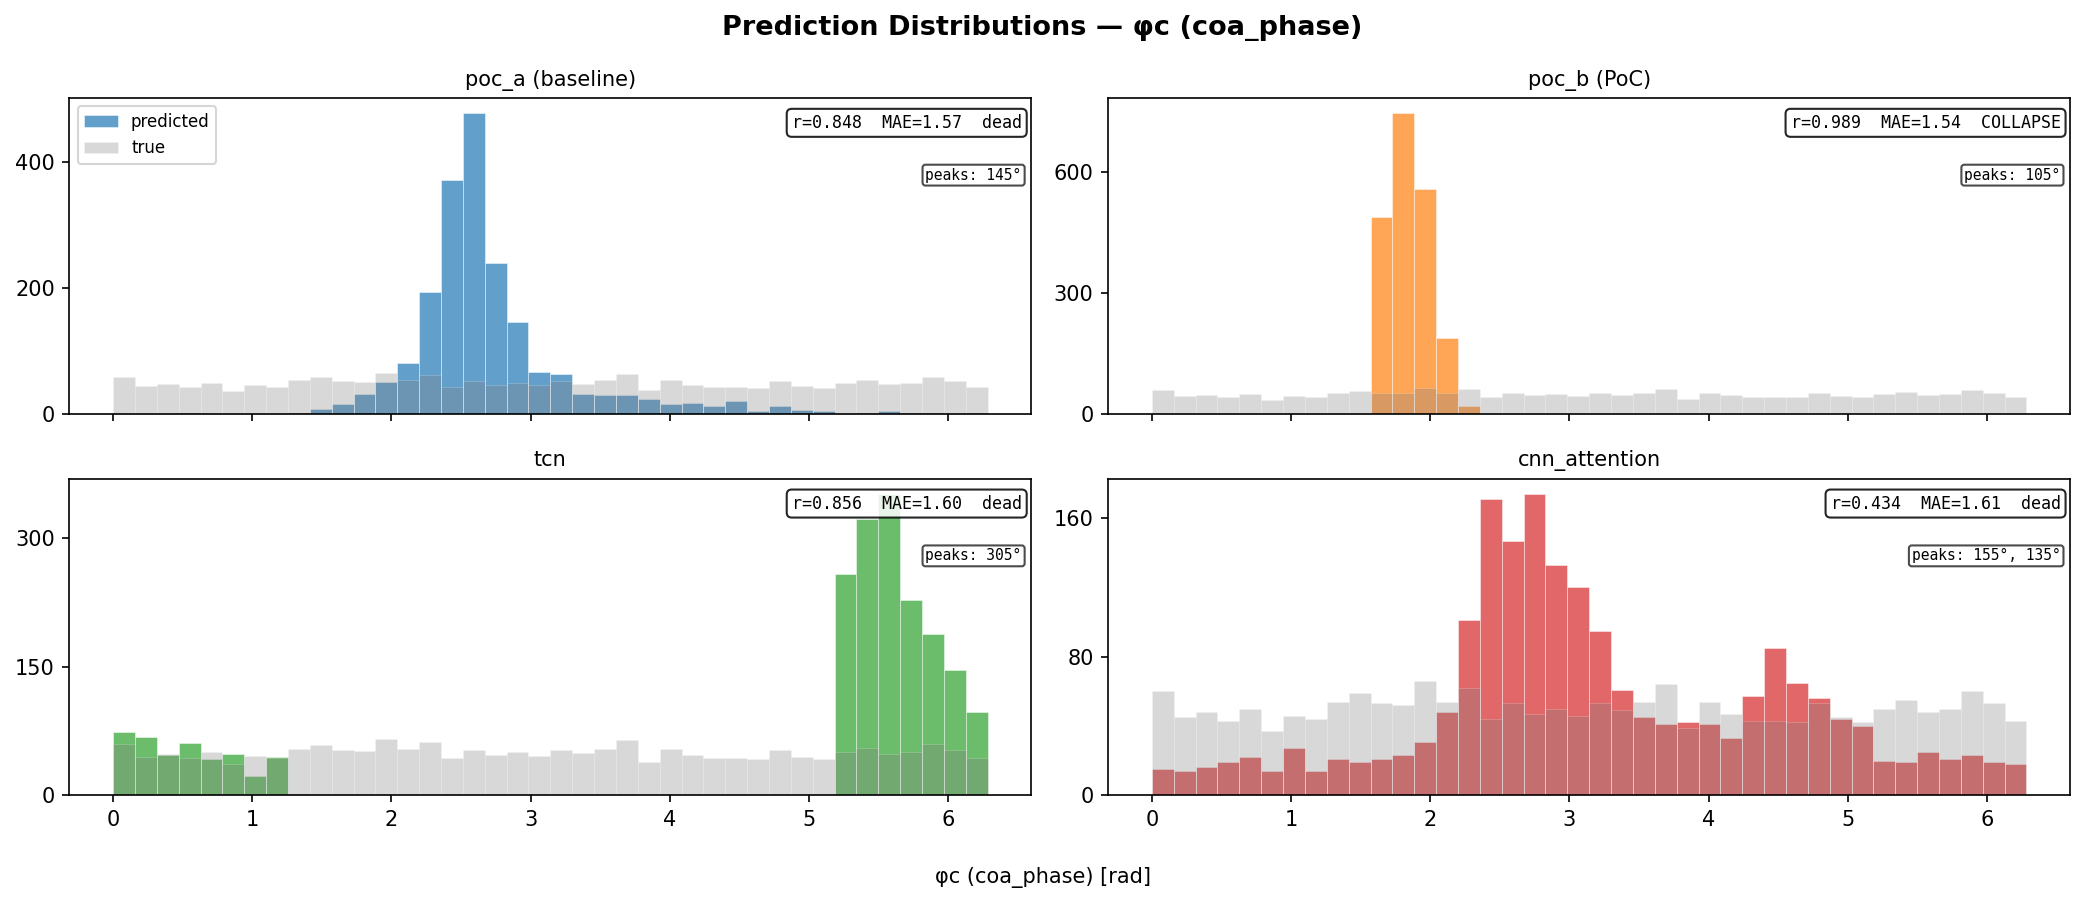
\includegraphics[width=\textwidth]{histogram_coa_phase_20260720_234304.png}
    \caption[Predicted $\varphi_c$ distributions]{Predicted $\varphi_c$ distributions (color) against the uniform truth (grey) for the four Run~7 models.
    Every model collapses to one or a few preferred angles ($r_{\mathrm{circ}} = 0.43$--0.99) while angular MAE sits at the null $\pi/2 \approx 1.571$ --- optimal constant-prediction behavior for an unidentifiable target.}
    \label{fig:phicpsi:hist}
\end{figure}

\subsection{Confound elimination}
\label{sec:phicpsi:confounds}

A five-section verification plan was executed against the Run~7 checkpoints under an explicit gating rule: nothing downstream counts as evidence about the degeneracy until the interpretability of the metrics themselves is established.
Table~\ref{tab:phicpsi:battery} summarizes.

\begin{table}[tbp]
    \centering
    \caption{Verification battery.}
    \label{tab:phicpsi:battery}
    \resizebox{\textwidth}{!}{
    \begin{tabular}{@{}lll@{}}
        \toprule
        Confound                            & Check                                 & Outcome                                                                                                                                                                                              \\
        \midrule
        Penalty silently inactive           & config $+$ code-path inspection       & $\lambda = 0.01$ confirmed active in all four configs                                                                                                                                                \\
        Magnitude drift invalidates metrics & full 80-epoch std\_ratio trajectories & 2/4 models fully healthy (poc\_b, cnn\_attention); tcn $\varphi_c$ still declining (0.34, $-0.0078$/epoch), poc\_a $\psi$ stable-but-low (0.44) $\to$ flagged, pursued in \S\ref{sec:phicpsi:prereg} \\
        Gradient path dead                  & perturbation $+$ gradient-chain trace & path healthy; an $89\times$ prediction-sensitivity asymmetry initially flagged, closed by the calibrated standalone trace's paired-statistic channel (\S\ref{sec:phicpsi:asymmetry})                                                                    \\
        poc\_b config bug                   & config diff vs poc\_a                 & four intentional keys only; worse collapse \emph{explained} by curriculum                                                                                                                            \\
        cnn\_attention hides real learning  & config diff $+$ architecture trace    & outlier metrics are attention-pooling variance artifacts; ang\_MAE at null                                                                                                                           \\
        Sub-null MAE is real signal         & 10{,}000-permutation bootstrap        & 11/12 model$\times$head tests non-significant; $\varphi_c$ and $\psi$: 0/8                                                                                                                           \\
        Learning hides in loud events       & SNR-tercile stratification            & no model--head pair shows a monotonic-and-material SNR trend                                                                                                                                         \\
        Ordering-confounded bootstrap       & row-order audit                       & data i.i.d.\ (window variance ratio 0.991); artifact bound 0.013\,rad                                                                                                                                \\
        \bottomrule
    \end{tabular}
    }
\end{table}

Two of these deserve narrative attention.

\paragraph{The poc\_b anomaly is supporting evidence, not a bug.}
The combination-space model collapsed \emph{more} severely than its baseline twin ($r_{\mathrm{circ}}$ 0.989 vs 0.848).
The config diff shows only the four intended poc-mode keys; the mechanism is the curriculum itself.
For near-face-on samples $w(\iota) \approx 0$ suppresses the poorly-constrained combination, so the model effectively trains one combination --- a single constraint on the two-dimensional $(\varphi_c, \psi)$ --- and the optimal response to a single unlearnable constraint under circular loss is a sharp constant, which is what poc\_b produces (a single peak carrying ${\sim}42\%$ of all predictions).
The design would have exploited a breakable degeneracy; its collapse into the constant predictor is what that design does when the degeneracy is not breakable.
(Cost: a mild, predictable transfer-interference tax on chirp mass, MAE $0.977 \to 1.024$.)

\paragraph{The cnn\_attention outlier is an artifact with a testable signature.}
Its lower $r_{\mathrm{circ}}$ comes from learned attention pooling producing higher-variance features than fixed GAP/GMP readouts --- spreading predictions without informing them (ang\_MAE 1.597, \emph{worst} of the four).
Its nominally significant inclination result is dissected below.

\subsection{Statistical significance}
\label{sec:phicpsi:bootstrap}

\begin{table}[tbp]
    \centering
    \caption{Label-permutation bootstrap ($N = 10{,}000$ shuffles,
        5{,}000 validation samples, one-sided). $z > 0$ means observed
        ang\_MAE beats the shuffled-null mean.}
    \label{tab:phicpsi:bootstrap}
    \small
    \begin{tabular}{@{}lccc@{}}
        \toprule
        Model          & $\varphi_c$: $z$, $p$ & $\psi$: $z$, $p$ & $\iota$: $z$, $p$         \\
        \midrule
        poc\_a         & $-0.20$, 0.579        & $+0.46$, 0.324   & $+1.04$, 0.152            \\
        poc\_b         & $-1.25$, 0.895        & $-0.05$, 0.518   & $+0.07$, 0.464            \\
        tcn            & $-0.56$, 0.712        & $-0.33$, 0.630   & $+1.21$, 0.114            \\
        cnn\_attention & $-2.43$, 0.994        & $+0.07$, 0.472   & $\mathbf{+3.17,\ 0.0007}$ \\
        \bottomrule
    \end{tabular}
\end{table}

Eleven of twelve tests are non-significant (Table~\ref{tab:phicpsi:bootstrap}); \textbf{all eight $\varphi_c/\psi$ tests fail}, six of them on the \emph{worse-than-shuffled} side.
The single nominal detection --- cnn\_attention on inclination --- does not survive scrutiny: its effect size is $\Delta = 0.038$\,rad ($2.2^\circ$), and the effect is uniform across SNR terciles (1.526/1.548/1.527) --- the signature of a population-level output-distribution bias, not of per-event information extraction; a genuinely strain-derived effect must grow with SNR.
A row-ordering audit additionally bounded the largest possible ordering artifact at 0.013\,rad and confirmed the permutation null is valid (validation data i.i.d.; window variance ratio 0.991).

\subsection{SNR stratification}
\label{sec:phicpsi:snr}

If weak phase information were present but diluted, it would concentrate in loud events.
It does not.
Across terciles (SNR $[7.0, 9.6]$ / $[9.7, 12.3]$ / $[12.3, 15.0]$, $n \approx 1{,}666$ each): every $\psi$ result lies within 0.007\,rad of the null in every tercile for every model; three of four models are non-monotonic in $\varphi_c$; the single monotonic case (tcn: $1.633 \to 1.557 \to 1.543$) has a high-SNR improvement of only 0.027\,rad --- beneath the 0.038\,rad artifact scale established in \S\ref{sec:phicpsi:bootstrap}, and produced by the one model whose $\varphi_c$ std\_ratio never converged (\S\ref{sec:phicpsi:prereg}), rendering it doubly uninterpretable as evidence of learning.

\subsection{Run 8: the $\lambda = 0$ ablation}
\label{sec:phicpsi:ablation}

One loose thread survived the battery: Run~7's validation circular losses \emph{rose} slightly over training ($+0.014$ to $+0.025$).
A rising loss could mean the magnitude penalty was actively corrupting predictions --- an engineering artifact worth fixing, not more null evidence --- so the two TCN-trunk baselines were re-run with $\lambda = 0$ (Fig.~\ref{fig:phicpsi:lam0}; Table~\ref{tab:phicpsi:lam0}).

\begin{table}[tbp]
    \centering
    \caption{Endpoint drift of validation circular loss.}
    \label{tab:phicpsi:lam0}
    \small
    \begin{tabular}{@{}llccl@{}}
        \toprule
        Model  & Head        & $\Delta$ at $\lambda{=}0$ & $\Delta$ at $\lambda{=}0.01$ & Reading                                      \\
        \midrule
        poc\_a & $\varphi_c$ & $+0.0010$                 & $+0.0249$                    & artifact of $\lambda$ (resolved)             \\
        poc\_a & $\psi$      & $+0.0002$                 & $+0.0163$                    & artifact of $\lambda$ (resolved)             \\
        tcn    & $\varphi_c$ & $+0.0011$                 & $+0.0204$                    & artifact of $\lambda$ (resolved)             \\
        tcn    & $\psi$      & $\mathbf{+0.0072}$        & $+0.0136$                    & persists at half size --- unexplained, small \\
        \bottomrule
    \end{tabular}
\end{table}

Three of four drift signals vanish with the penalty off: the creep was a penalty/uncertainty-weighting interaction, not anti-learning.
The fourth (tcn $\psi$) persists at $+0.0072$ on a loss of ${\sim}1.0$ and is recorded as unexplained-but-small rather than forced into the majority pattern.
The ablation also confirmed it was genuinely an off-state --- without the penalty, std\_ratio diverged to 73--83 --- and final MAEs at $\lambda = 0$ landed on the same nulls as every other run ($\varphi_c \approx 1.579$; $\psi \approx 0.780$--0.785).

\begin{figure}[tbp]
    \centering
    \includegraphics[width=\textwidth]{lam0_ablation_trajectories.png}
    \caption[$\lambda = 0$ ablation]{$\lambda = 0$ ablation for poc\_a and tcn: validation/training circular loss and validation std\_ratio for $\varphi_c$ (top) and $\psi$ (bottom); $\lambda = 0$ (solid) vs the $\lambda = 0.01$ references (dashed).
    Removing the penalty eliminates the upward validation-loss drift (e.g.\ $+0.0010$ vs $+0.0249$ for poc\_a $\varphi_c$) but lets $\lVert\mathbf{v}\rVert$ diverge (std\_ratio $> 140$ at peak).
    Circular loss remains at $\approx 1.0$ in every configuration.}
    \label{fig:phicpsi:lam0}
\end{figure}


\subsection{Closing the last open probe: the $89\times$ sensitivity asymmetry}
\label{sec:phicpsi:asymmetry}

Verification item A.3 left one mechanistic loose end: after a single optimizer step, the periodic heads' predictions moved with relative change ${\sim}1.6 \times 10^{-2}$, some $89\times$ more than the converged chirp-mass head's $1.8 \times 10^{-4}$ --- movement a one-step snapshot cannot classify as slow learning or noise.
The multistep trace built to resolve this was gated behind the pre-registered stability gate and therefore never ran during the retune; after the retune closed, it was decoupled into a standalone script and executed against the Run~7 checkpoints (25 consecutive gradient steps on a fixed 128-sample batch, with predictions tracked on a disjoint 512-sample probe).

\begin{table}[tbp]
    \centering
    \caption{Standalone multistep perturbation trace, at the converged checkpoints (``final'') and after a fresh initialization plus ${\sim}$1-epoch warmup (``early'').
        net/sum is the ratio of net displacement to summed per-step displacements (random-walk reference $1/\sqrt{25} = 0.20$).
        $\Delta$ is the paired per-sample probe change over the 25 steps with its paired-SE $t$ statistic --- circular loss for $\varphi_c/\psi$, transformed-target MSE for mchirp.}
    \label{tab:phicpsi:trace}
    \small
    \begin{tabular}{@{}llccc@{}}
        \toprule
        Stage & Model & $\varphi_c$: net/sum, $\Delta$ ($t$) & $\psi$: net/sum, $\Delta$ ($t$) & mchirp: net/sum, $\Delta$ ($t$) \\
        \midrule
        final & poc\_a         & 0.30, $-0.018$ ($-0.9$) & 0.63, $+0.043$ ($+0.8$) & 0.04, $+0.021$ ($+4.2$) \\
        final & poc\_b         & 0.39, $-0.013$ ($-1.0$) & 0.23, $+0.004$ ($+1.7$) & 0.04, $+0.040$ ($+9.0$) \\
        final & tcn            & 0.92, $-0.010$ ($-0.2$) & 0.36, $+0.050$ ($+1.6$) & 0.03, $+0.017$ ($+4.3$) \\
        final & cnn\_attention & 0.41, $-0.044$ ($-1.1$) & 0.34, $+0.023$ ($+0.7$) & 0.19, $+0.065$ ($+4.4$) \\
        early & poc\_a         & 0.16, $-0.017$ ($-1.6$) & 0.14, $+0.004$ ($+0.1$) & 0.09, $\mathbf{-0.158}$ ($\mathbf{-5.2}$) \\
        early & poc\_b         & 0.08, $-0.006$ ($-0.7$) & 0.09, $+0.001$ ($+0.1$) & 0.13, $\mathbf{-0.129}$ ($\mathbf{-3.4}$) \\
        early & tcn            & 0.24, $-0.002$ ($-0.0$) & 0.15, $+0.035$ ($+0.6$) & 0.10, $\mathbf{-0.113}$ ($\mathbf{-4.1}$) \\
        early & cnn\_attention & 0.42, $+0.001$ ($+0.0$) & 0.37, $-0.031$ ($-0.6$) & 0.29, $\mathbf{-0.646}$ ($\mathbf{-8.5}$) \\
        \bottomrule
    \end{tabular}
\end{table}

Two observations (Table~\ref{tab:phicpsi:trace}) stand on arithmetic alone.
First, the asymmetry is real and now explained: the periodic heads' raw outputs move coherently and far (net/sum up to 0.93 against the 0.20 random-walk reference), while the converged scalar control barely moves net (net/sum 0.03--0.16; its positive cosine similarity is attributable to Adam momentum, which correlates consecutive steps for every head).
Second, the coherent movement is dominantly \emph{radial}, not angular: the circular loss depends only on the predicted angle, and its change over 25 steps is bounded by $|\Delta| \le 0.051$ on a loss of ${\approx}1.0$ while the raw displacement is a large fraction of the output norm --- large coherent raw movement with near-zero angular consequence is precisely the $\lVert\mathbf{v}\rVert$-magnitude dynamics of \S\ref{sec:phicpsi:pathology2}, and the two most directional cases (tcn/$\varphi_c$, poc\_a/$\psi$) are exactly the two heads with the known std\_ratio pathologies.

The first run of the trace was reviewed before acceptance, and the review reshaped the instrument itself; the sequence is reported in order because each step gates the next.
The review raised two objections: the positive control had failed --- mchirp, the best-learned head in the investigation ($R^2 \approx 0.96$ throughout), read AMBIGUOUS at every converged checkpoint, so the classifier could not distinguish a demonstrably learned head from a dead one --- and the probe-loss deltas lacked the correct \emph{paired} statistic (the first run recorded only means, and a marginal-SE comparison is invalid for a before/after change on the same fixed samples).
Both were remediated: per-sample paired statistics were added to the instrument, and a calibration stage was defined with a pre-stated criterion --- rerun the trace near the start of training (fresh initialization plus ${\sim}$1-epoch warmup, since per-epoch checkpoints were never saved), where a genuinely learning mchirp \emph{must} read directional, with failure defined to retire the classifier.

\textbf{The calibration failed its criterion --- and in failing, validated the measurement that matters.}
Early-stage mchirp never read directional (net/sum 0.09--0.29) \emph{while its probe MSE was collapsing at $t = -3.4$ to $-8.5$}, the strongest learning signal in the entire table: the displacement-geometry classifier labels the fastest-learning head ``noise-like.''
The mechanism is instructive --- learning is not rigid drift; per-step prediction deltas decorrelate as different samples' errors are corrected --- and the verdict is mechanical: per the pre-stated tree, the geometry classifier is retired and no directional/ambiguous verdict from either run is used.
The same run, however, constitutes a \emph{passed} positive control for the instrument's other channel: the paired probe-loss statistic detects early mchirp learning decisively in all four models, and on that validated channel every periodic head is null at both stages (early $|t| \le 1.6$, final $|t| \le 1.7$, signs mixed across models and heads).
The early stage is the sharper result: a within-run, stage-matched, positive-controlled contrast in which the same instrument, over the same 25 steps, watches mchirp learn steeply while $\varphi_c$ and $\psi$ sit at the random baseline.
The paired statistic also extinguishes the one nominal escalation trigger from the first run --- tcn/$\varphi_c$, directional at net/sum 0.92 with an apparently decreasing probe loss, measures $-0.0097 \pm 0.0491$ ($t = -0.20$) --- and the radial explanation of the original $89\times$ asymmetry stands on arithmetic independent of the retired classifier: raw periodic outputs move by a large fraction of their norm while the angular loss moves by at most $|0.051|$, and the two largest raw movers are the two known std\_ratio-pathology heads.

Two secondary observations complete the account.
First, the final-stage mchirp deltas are significantly \emph{positive} --- probe MSE worsens by $+0.017$ to $+0.065$ ($t = +4.2$ to $+9.0$) --- which is not a probe artifact but the expected signature of resuming training on a single fixed batch: at convergence the full-data gradient is ${\approx}0$ while the batch gradient is not, so 25 repeated steps move the head along batch-specific directions at the expense of the held-out optimum.
Three pieces of in-hand evidence support this reading over a data-loading quirk: the probe pipeline is stage-independent yet yields strongly negative deltas early and positive ones late; the gradient batch is disjoint from the probe by construction, so the degradation is genuine out-of-batch generalization loss; and the effect appears only on the head with a real strain-to-target mapping --- a converged optimum to be dragged away from.
Read as an unplanned second control, it strengthens the final-stage null: the paired channel demonstrably has the power to detect a real, if artifactual, effect at the converged stage --- and $\varphi_c/\psi$ still show nothing against that backdrop.
Second, on sensitivity: the per-combo minimum detectable effect (${\approx}2\times$ the paired SE) spans ${\approx}0.005$--$0.10$ loss units across the twelve cases, so the individual $\varphi_c/\psi$ point estimates (up to $|0.050|$) are non-significant partly because the single-batch probe design yields wide standard errors --- the final-stage per-combo null is ``not rejected and bounded at the few-percent level,'' not ``excluded to arbitrary precision.''
This is adequate for A.3's mechanistic role: the degeneracy verdict itself is carried independently by the $N = 10{,}000$ label-permutation bootstrap and the SNR stratification, not by this trace.

\textbf{A.3 is closed}: the $89\times$ asymmetry was radial movement without angular learning.
The disposition honors the pre-stated decision tree in order --- the calibration criterion failed, so the classifier it governed is retired --- and the closure is then re-founded, transparently post hoc, on the surviving channel, which carries its own passed control from the same run; that residual caveat is recorded in the threats-to-validity list rather than hidden.


\section{The Pre-Registered $\lambda$ Retune}
\label{sec:phicpsi:prereg}

\subsection{Why pre-register an engineering sweep}
\label{subsec:why-pre-register-an-engineering-sweep}

After \S\ref{sec:phicpsi:results}, two model--head pairs remained \emph{formally uninterpretable} rather than cleanly null: tcn/$\varphi_c$ (std\_ratio still declining at $\lambda = 0.01$) and poc\_a/$\psi$ (stable but below the healthy band).
The obvious next step --- raise $\lambda$ and see whether the numbers ``look better'' --- is precisely the kind of after-the-fact eyeballing that had already misled this investigation three times (the $R^2 = 0.75$ collapse artifact; an endpoint-only std\_ratio summary that concealed a mid-training crash-and-recovery; the Run~8 drift artifact).
The decision criteria were therefore \textbf{locked in writing before any retune ran}~\cite{nosek2018preregistration}, with the verdict computed mechanically by the diagnostic scripts, not by inspection:

\begin{description}
\item[Scope.]
Exactly two primary tests: tcn/$\varphi_c$ and poc\_a/$\psi$.
All else exploratory, with promotion to ``primary'' after the fact explicitly forbidden.
\item[Step 0 --- interpretability gate.] std\_ratio healthy iff ${<}10\%$ of the final 40 epochs fall outside $[0.5, 2.0]$ \emph{and} the linear trend over those epochs is within $\pm 0.005$/epoch.
Failure at $\lambda = 0.05$ $\to$ try $\lambda = 0.10$; failure at both $\to$ report ``$\lambda$ alone insufficient,'' counted \textbf{neither as null nor as counter-evidence}.
\item[Step 1 --- significance.]
The \S\ref{sec:phicpsi:bootstrap} bootstrap, Bonferroni-corrected for two tests ($p < 0.025$).
\item[Step 2 --- effect-size floor.]
$\Delta$ang\_MAE $\ge 0.10$\,rad ($\approx 5.7^\circ$) --- set $\approx 3\times$ above the largest known metric artifact (0.038\,rad) and $\approx 8\times$ above the ordering bound (0.013\,rad).
\item[Step 3 --- SNR consistency.]
Improvement monotonic non-decreasing across terciles, with the high-SNR tercile independently clearing the floor.
\end{description}

Only a result passing all four steps would count as counter-evidence to the degeneracy hypothesis.

\subsection{Outcome}\label{subsec:outcome}

\begin{table}[tbp]
    \centering
    \caption{Pre-registered gate results.}
    \label{tab:phicpsi:gates}
    \small
    \begin{tabular}{@{}clccl@{}}
        \toprule
        $\lambda$ & Test              & frac.\ unhealthy (last 40 ep) & trend /epoch         & Gate                       \\
        \midrule
        0.05      & tcn / $\varphi_c$ & 0.05 \checkmark               & $-0.0064$ $\times$   & \textbf{FAIL}              \\
        0.05      & poc\_a / $\psi$   & 0.35 $\times$                 & $+0.0072$ $\times$   & \textbf{FAIL}              \\
        0.10      & tcn / $\varphi_c$ & 0.28 $\times$                 & $-0.0026$ \checkmark & \textbf{FAIL} (worse)      \\
        0.10      & poc\_a / $\psi$   & 0.73 $\times$                 & $+0.0073$ $\times$   & \textbf{FAIL} (much worse) \\
        \bottomrule
    \end{tabular}
\end{table}

At $\lambda = 0.05$ both failures were near-misses with a shared shape --- each trajectory settles into a healthy plateau (0.58--0.62 and 0.53--0.56 respectively) only in the last 15--20 epochs, and the 40-epoch window still contains the climb into that band (Fig.~\ref{fig:phicpsi:lam005}).
At $\lambda = 0.10$ the failures were not near-misses and diverged in character: poc\_a/$\psi$ crashes through epochs ${\sim}30$--48 and is still recovering at epoch 80 (crossing 0.5 only in the final 11 epochs), while tcn/$\varphi_c$ oscillates across $[0.2, 0.95]$ with no convergence at all (Fig.~\ref{fig:phicpsi:lam010}).
The exploratory pairs mostly regressed too: $\lambda = 0.10$ helped none of the four TCN-trunk head/model combinations and worsened three.
Throughout all of it, circular loss stayed at 1.004--1.008 --- flat at the null, as in every preceding run.

\begin{figure}[tbp]
    \centering
    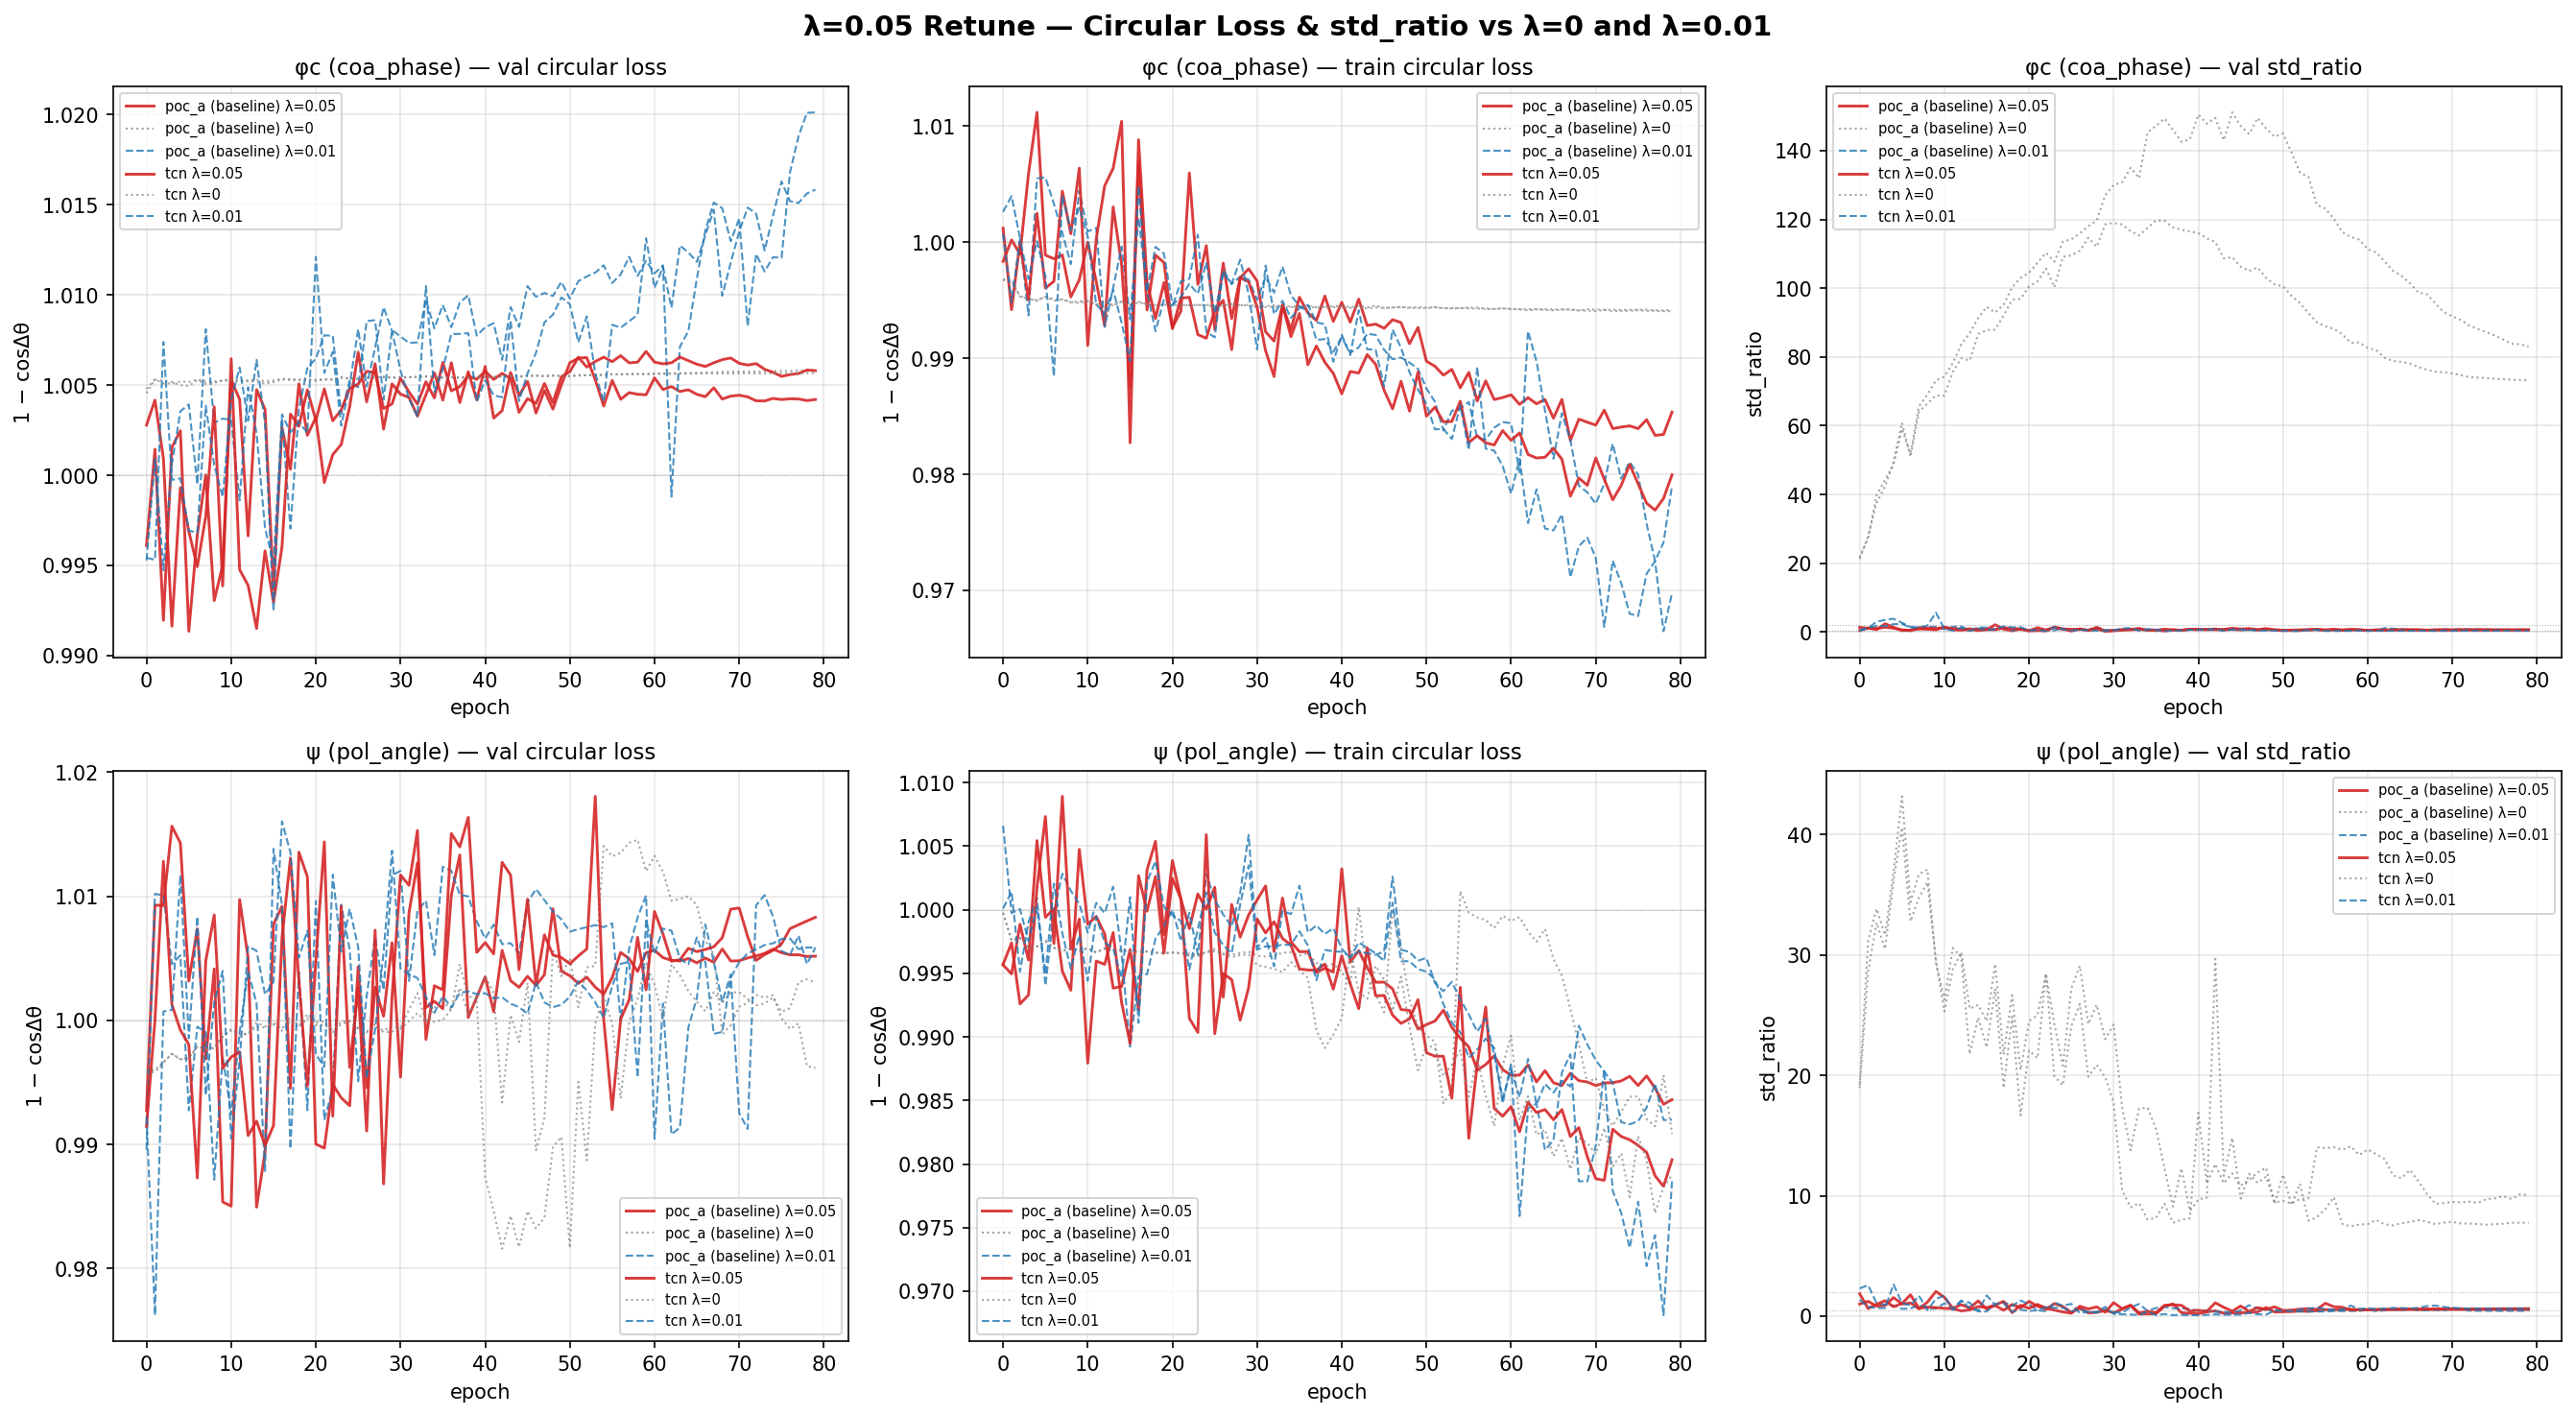
\includegraphics[width=\textwidth]{lam005_retune_trajectories.png}
    \caption[Run 9a, $\lambda = 0.05$ retune]{Run~9a, $\lambda = 0.05$,
        overlaid on $\lambda = 0$ and $\lambda = 0.01$ . The penalty
        holds std\_ratio at order unity, but neither pre-registered target
        passes the stability gate, and validation circular loss remains at
        $\approx 1.0$.}
    \label{fig:phicpsi:lam005}
\end{figure}

\begin{figure}[tbp]
    \centering
    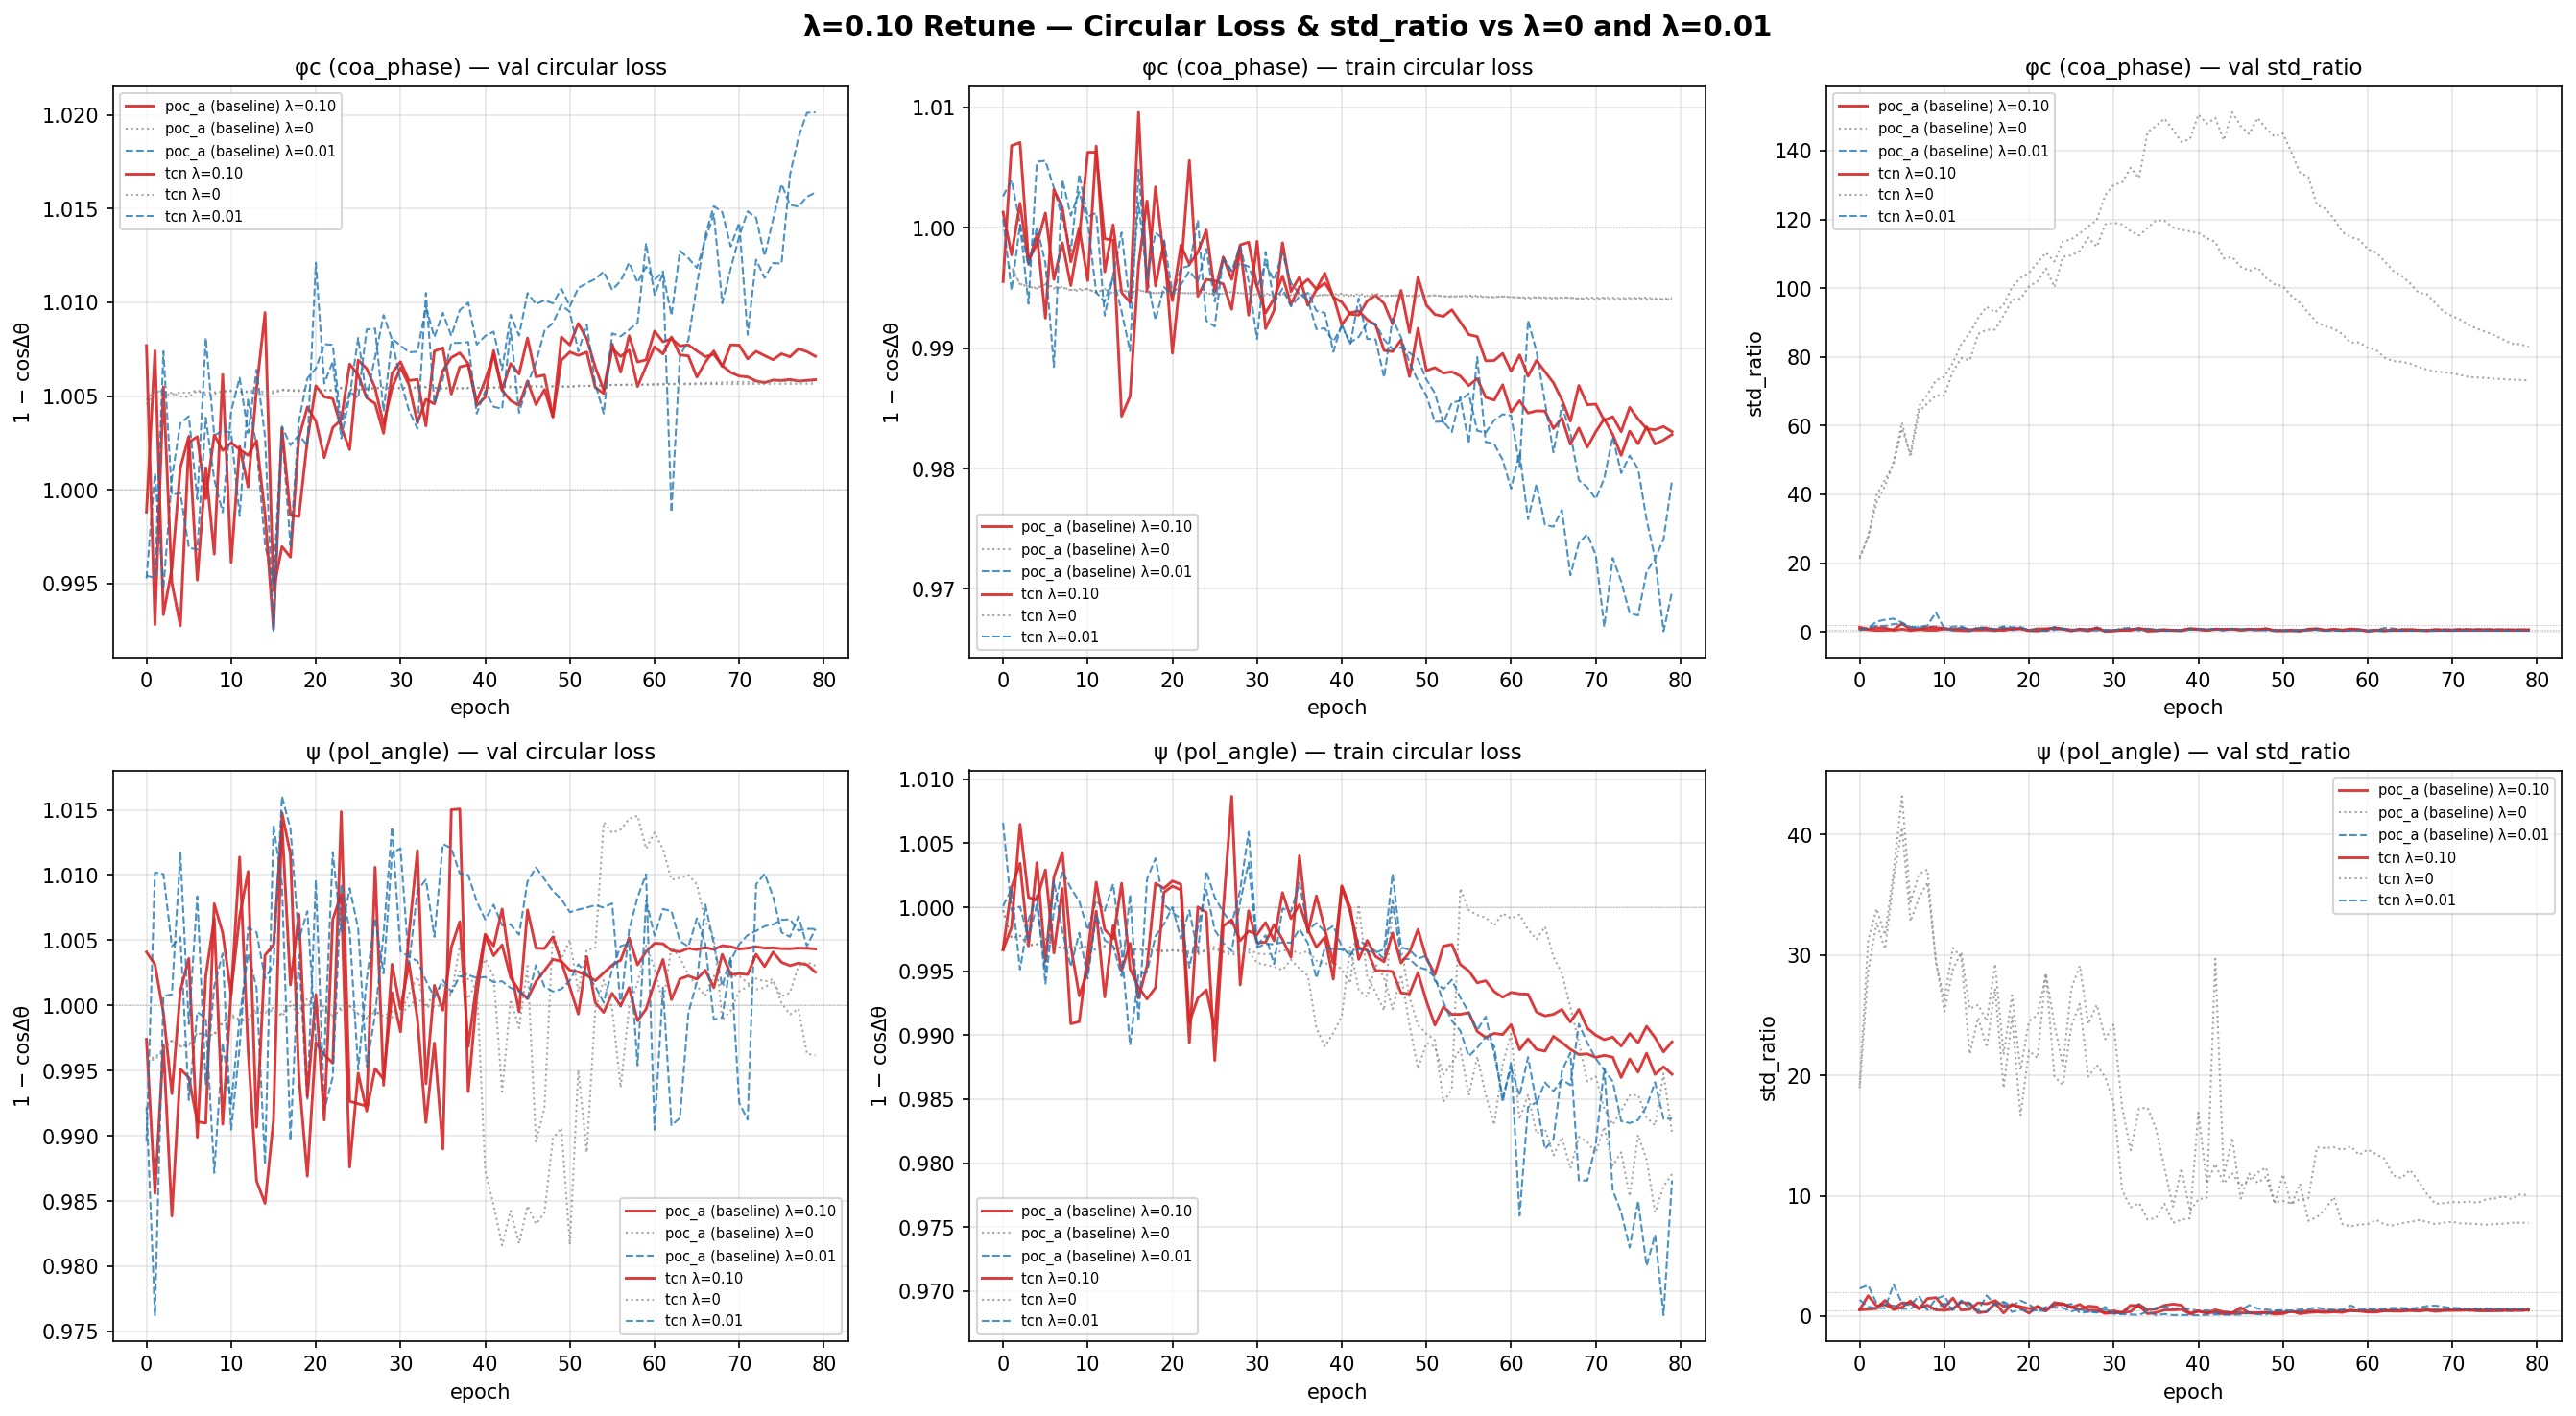
\includegraphics[width=\textwidth]{lam010_retune_trajectories.png}
    \caption[Run 9b, $\lambda = 0.10$ retune]{Run~9b, $\lambda = 0.10$,
        same layout. The stronger penalty fails the gate more severely
        (poc\_a/$\psi$: 73\% of late epochs unhealthy) while circular loss
        stays at the random-guessing plateau.}
    \label{fig:phicpsi:lam010}
\end{figure}

\subsection{Verdict}\label{subsec:verdict}

Per the pre-registered decision table --- applied as written, not re-derived after seeing the data --- the result is: \textbf{$\lambda$ alone is insufficient to stabilize std\_ratio for either primary target}; the $\lambda$-sweep $\{0, 0.01, 0.05, 0.10\}$ is exhausted; any further pursuit is architecture-level.
One observation sits outside the pre-registered frame but belongs in the record: the response to $\lambda$ is \emph{peaked}, not monotonic --- $\lambda = 0.05$ produced near-misses on both targets while $\lambda = 0.10$ regressed on every head/model combination --- so ``exhausted'' refers to the pre-registered sweep and its stopping rule, not to the $\lambda$ dimension as such.
A finer, freshly pre-registered mini-sweep over $\lambda \in [0.02, 0.08]$ plausibly contains a stability optimum; it was not pursued here for reasons of time and is recorded as future work (\S\ref{sec:phicpsi:future}) rather than claimed to be ruled out.
The two pairs are filed as \emph{uninterpretable}, not as additional nulls and not as counter-evidence.
Steps 1--3 never executed for any configuration, at any $\lambda$ --- which is itself a summary statistic of the whole investigation: \textbf{no result ever cleared even the first gate of a pre-declared path to counter-evidence.}

Two disciplined refusals are worth recording.
The gate's 40-epoch window is arguably miscalibrated for the plateau learning-rate schedule's late settling --- a real concern, flagged during Run~9a --- but revising a criterion between pre-registered arms, with results in hand, would reintroduce exactly the flexibility pre-registration exists to remove; the question is documented for future gates instead.
And the near-miss $\lambda = 0.05$ trajectories \emph{look} healthy at endpoint --- the temptation to wave them through was declined for the same reason.


\section{Discussion}
\label{sec:phicpsi:discussion}

\subsection{What the evidence supports}\label{subsec:what-the-evidence-supports}

The degeneracy hypothesis --- $\varphi_c$ and $\psi$ carry no strain-only recoverable signal for this population in this architecture/loss family --- is the best-supported reading of nine training campaigns:
\begin{enumerate}
\item validation circular loss flat at the random value $\approx 1.0$ in every run, every model, every $\lambda$, with healthy gradients and unit-scale magnitudes over the second half of training in the clean models;
\item 0 of 8 $\varphi_c/\psi$ bootstrap tests significant (11 of 12 overall), with the single scalar-head detection explained as a population bias;
\item no SNR-dependent improvement anywhere --- the direction any real strain-derived effect must point;
\item the combination-space model, purpose-built to exploit the analytically confirmed conditioning structure of \S\ref{sec:phicpsi:prereq}, collapsing \emph{into} the constant predictor exactly as it should if the residual per-sample information is nil;
\item positive controls learned to high fidelity from the same features throughout.
\end{enumerate}

Two points sharpen what is and is not being claimed.
First, the claim is \emph{conditional}: it applies to point-estimating regression on this SNR-7--15, two-detector, dominant-mode population, under circular loss --- not to Bayesian posterior recovery (a sampler still recovers a meaningful \emph{joint} posterior over $(\varphi_c, \psi)$), not to louder signals, not to alternative data representations (e.g.\ frequency-domain or time--frequency inputs), and not to configurations with inclination supplied as side information (\S\ref{sec:phicpsi:future}).
Second, the analytic study of \S\ref{sec:phicpsi:prereq} makes the null \emph{informative} rather than merely disappointing: a combination-conditioning ratio of only ${\sim}1.16\times$ population-averaged --- concentrated face-on, where the curriculum then down-weights it to zero --- quantifies how little marginal structure there was for a per-event point estimator to find.
The networks did not miss an obvious target; they confirmed, at scale, how small the target is.

\subsection{Sufficiency of the architecture pool}
\label{sec:phicpsi:pool}

A natural objection to any architecture-crossed null is: \emph{why only seven models?}
The answer is that architecture count is the wrong axis for defending this particular claim, and the design reflects that deliberately.

A comparative claim (``architecture $X$ is best for task $Y$'') grows stronger with breadth, and every untried model is a hole in it.
A null of the form ``the input--label relationship carries no recoverable signal'' does not: it grows stronger with \emph{diversity of inductive bias} and with \emph{mechanism-level evidence}, both of which saturate quickly.
On the first, the five trunk families (\S\ref{sec:phicpsi:trunks}, Table~\ref{tab:phicpsi:trunks}) span qualitatively different hypotheses about how phase information could be encoded --- long-range dilated convolution, local hierarchical convolution, content-based attention, explicit multi-scale filtering, and deep residual composition --- rather than five samples from one family.
On the second, the decisive observation is that \textbf{capacity was demonstrably not the binding constraint}: the higher-capacity trunks drove \emph{training} circular loss down to ${\approx}0.49$--$0.60$ while validation loss stayed pinned at 1.0 (Fig.~\ref{fig:phicpsi:comboloss}).
That is precisely what added capacity does against an uninformative target --- it memorizes.
An eighth architecture buys another memorization curve, not information absent from the strain; once the failure is localized in the data by flat validation loss under certified-healthy gradients, in agreement with the analytic degeneracy of \S\ref{sec:phicpsi:prereq}, architecture search has no remaining expected payoff.
In one sentence: \emph{the null is a statement about the data, not about the hypothesis class, and the memorization gap is the evidence that the hypothesis class was not the limit.}

The progressive narrowing of the pool --- seven configurations, then four, then two --- likewise reflects criteria, not attrition.
The seven were never seven independent tests but five trunks plus the two head parameterizations on the primary trunk; the cut to four (poc\_a, poc\_b, tcn, cnn\_attention) selected the $\lambda$-matched subset after the magnitude penalty was introduced (\S\ref{sec:phicpsi:protocol}), the remaining three trunks retaining evidential value as unmatched corroboration; and the cut to the two \emph{certified-clean} models (poc\_b, cnn\_attention) was imposed by the pre-declared std\_ratio interpretability gate (\S\ref{sec:phicpsi:confounds}), not by preference among results.
Each restriction is documented and criterion-based, and the excluded configurations agree with the included ones at every point where they can be compared.

For the same reason, the deliberate decision \emph{not} to expand the architecture pool in future work (\S\ref{sec:phicpsi:future}) is scoping rather than omission: the evidence localizes the failure in the information available to the network, so the productive next lever is conditioning information ($\iota$-conditioning), not a broader model zoo.
A single modern-family spot-check (e.g.\ a state-space sequence model at $\lambda = 0.01$) would be a cheap robustness supplement, but per unit of compute, seed replication of an existing configuration addresses a larger residual risk (\S\ref{sec:phicpsi:threats}) than any additional architecture.

\subsection{Threats to validity}
\label{sec:phicpsi:threats}

We record the limitations explicitly, in roughly descending order of concern.
\begin{itemize}
\item \textbf{Two configurations remain uninterpretable.} tcn/$\varphi_c$ and poc\_a/$\psi$ never achieved certified metric health at any $\lambda$; the clean degeneracy test rests on poc\_b and cnn\_attention (plus the ablation and pre/post-fix consistency of every other configuration).
The null is multiply corroborated, but its \emph{certified} base is narrower than its table count.
\item \textbf{The A.3 closure rests on a within-run-validated channel.}
The trace's pre-stated displacement-geometry classifier failed its positive control at calibration and was retired (\S\ref{sec:phicpsi:asymmetry}); the closure rests on the paired probe-loss statistic, whose own control passed emphatically in the same run (early mchirp $|t| = 3.4$--$8.5$) but which was added on review rather than pre-registered.
The evidence is positive-controlled; the channel choice is post hoc --- recorded here rather than hidden.
\item \textbf{Residual anomalies.} tcn/$\psi$'s $+0.0072$ validation-loss drift at $\lambda = 0$ remains unexplained (small, on a loss of ${\sim}1.0$); the inclination head's failure mechanism (Huber path, no normalization) is documented as distinct but is itself unresolved; and a sky-position degradation specific to the \texttt{SumDiffTrainer} runs ($8.2^\circ$--$10.0^\circ$ vs $3.3^\circ$--$4.5^\circ$ for the plain baselines) was flagged in the record but never investigated --- a known open issue, out of scope for this chapter.
\item \textbf{Design constraints.}
Single seed (42) per configuration --- replication is across architectures and $\lambda$ values, not across seeds; the five-trunk comparison is not $\lambda$-matched (three trunks trained at $\lambda = 0$), though the four models carrying the verified null are matched; the curriculum used the analytic $\sin^2\iota$ weight, not the Jacobian-fitted variant it was validated against; fixed 80-epoch budget with no early stopping; a single simulated dataset with a single noise realization per event.
\item \textbf{Metric-versioning note.}
Two evaluation passes over the Run~7 checkpoints differ by up to 0.026\,rad in periodic ang\_MAE (both straddling the same null; no verdict affected).
Tables~\ref{tab:phicpsi:prepost} and~\ref{tab:phicpsi:bootstrap} use the self-consistent bootstrap/stratification set.
\end{itemize}
None of these, alone or jointly, provides a mechanism by which a real, useful $\varphi_c/\psi$ signal could have hidden from all of \S\ref{sec:phicpsi:results} --- but they bound the strength of the claim honestly.

\subsection{Methodological lessons}\label{subsec:methodological-lessons}

Three transferable lessons emerge from the diagnostic arc, and they are the part of this chapter most likely to outlive its specific numbers.

\paragraph{Aggregate metrics are not evidence until their mechanism is verified.}
Every major error in this investigation was a plausible reading of a true number: $R^2 = 0.75$ (mode collapse in disguise), an endpoint std\_ratio of 0.62 (concealing a crash to 0.07 and recovery), rising validation loss (a regularizer interaction), a ``significant'' $p = 0.0007$ (population bias).
The correctives were never better metrics but mechanism inspection: forward-pass dumps, gradient-chain traces, full trajectories, code-level loss-path audits.
For null results especially, the epistemic burden inverts: a \emph{flat} loss is only informative once the gradient path that would have moved it is certified live.

\paragraph{Controls must be validated at the code level.}
The inclination head's coincident failure was, for a time, load-bearing evidence for a shared-mechanism (hence fixable, hence non-physical) explanation.
It shared the encoding, the architecture, and the failure signature --- but not, it turned out, the loss path.
A control that resembles the treatment in every visible metric can still differ in the one line of code that matters.

\paragraph{Pre-registration has a place inside engineering loops, not just at study level.}
The $\lambda$ retune's gates were written down precisely because the investigators had watched themselves misread results three times.
The payoff was concrete: a near-miss that endpoint-eyeballing would have waved through was held to the written criterion, a mid-stream temptation to recalibrate the gate was resisted and documented instead, and the final filing --- ``neither null nor counter-evidence'' --- is a category that post-hoc reasoning almost never produces but that honest accounting sometimes requires.

\subsection{Future work}
\label{sec:phicpsi:future}

Three successors are scoped, in priority order.
(i)~\textbf{Inclination conditioning}: supply true $(\sin\iota, \cos\iota)$ as an auxiliary input --- the analytic structure of \S\ref{sec:phicpsi:prereq} says the well-constrained combination is knowable \emph{given} $\iota$, so this tests whether the degeneracy is breakable with side information; a full implementation plan exists (train-time truth, with inference-time $\iota$ estimation explicitly out of scope).
(ii)~An \textbf{architecture-level attack on the std\_ratio instability} for the two uninterpretable pairs (the pre-registered $\lambda$-sweep's named next lever), or an explicit decision to close that thread; alongside it, a finer freshly pre-registered $\lambda$ mini-sweep over $[0.02, 0.08]$, motivated by the peaked $\lambda$-response observed in \S\ref{sec:phicpsi:prereg}.
(iii)~A \textbf{posterior-estimation reformulation}: the natural follow-on from ``point estimation is hopeless'' is not resignation but a conditional-density head (e.g.\ a von Mises mixture over the well-constrained combination), which the present chapter's null both motivates and baselines.


\section{Conclusion}
\label{sec:phicpsi:conclusion}

We set out to determine whether the coalescence phase and polarization angle of compact-binary signals are recoverable from strain by direct neural regression, individually or in their physically motivated sum/difference combinations.
After eliminating two genuine optimization pathologies that initially masqueraded as (and then obscured) the answer --- $\tanh$ saturation at initialization, and magnitude drift induced by a norm-blind circular loss --- and after subjecting the resulting flat learning curves to a verification battery spanning configuration audits, permutation tests, population stratification, an ablation, and a pre-registered two-arm regularization sweep, the answer is: \textbf{no}.
Every model, at every capacity and every regularization strength, converged to the optimal constant predictor, at the analytic random-guessing error, while learning four other parameters well from the same shared representation --- and no result at any point cleared even the first gate of a pre-declared path to counter-evidence.
The degeneracy is effectively exact for this population as a point-estimation problem.
The value of the chapter lies as much in the demonstrated discipline --- mechanism before metrics, code-validated controls, pre-registered criteria inside the engineering loop --- as in the null it certifies, and both carry directly into the inclination-conditioned and posterior-based formulations that follow.
